\section{Experiments and Evaluation}
\label{s:eval}
We divide our experiments into two different sections. In the first section, we give performance evaluation information on our trained autoencoder wireless networks. Next, we discuss how our implemented covert models perform in single-user and multi-user systems in terms of robustness to different channel models, data rates, and number of users.

\begin{figure*}[!tp]
	\center
	\begin{subfigure}{0.28\textwidth}
		\includegraphics[width=\linewidth]{figs/autoencoder_bler_awgn}
		\caption{AWGN channel}
	\end{subfigure}
	\begin{subfigure}{0.28\textwidth}
		\includegraphics[width=\linewidth]{figs/autoencoder_bler_rayleigh}
		\caption{Rayleigh fading channel}	
	\end{subfigure}
	\begin{subfigure}{0.28\textwidth}
		\includegraphics[width=\linewidth]{figs/autoencoder_bler_rician}
		\caption{Rician fading channel}	
	\end{subfigure}
	\caption{Autoencoders performance in terms of BLER over a range of SNR values in our single-user system. Models are trained over AWGN, Rayleigh and Rician fading channels for a set of parameters that has the same data rate.}
	\label{fig:autoencoder_bler}
\end{figure*}

\subsection{Baseline Single-User Autoencoder's Performance}
We implemented an autoencoder communication network for the normal communication between UserRX and UserTX. An \(Autoencoder (n, k)\) is a neural network communication model that sends \(k\) bits of data in \(n\) channel uses. For our results to be comparable with the original paper \cite{o2017introduction}, we choose our default parameters to be 8 and 4 for the number of channel uses and the binary message size, respectively. That said, we also evaluate our models for two other sets of parameters. All three sets of parameters have the same data rate but differ in number of channel uses. This gives us an intuition about how increasing number of channel uses or in other words, channel dimensionality, would affect the communication performance. In order to train our autoencoder model, we generate two datasets for training and testing by generating random binary messages \(s\) of size \(k\). Specifically, there are 8192 random binary messages in the training set and 51200 random binary messages in the test set. We intentionally created a much larger data set for testing to make sure that each symbol \(y\) undergoes various channel distortions to have an accurate evaluation of the model's performance. We set the learning rate to 0.001 and optimized the model using the Adam optimizer \cite{kingma2014adam}. We choose the batch size to be 1024 and train the model for 100 epochs. For the channel configuration, \textbf{we choose a fixed signal-to-noise ratio (SNR) value during training but evaluation is on a range of SNRs}. The SNR value for the AWGN channel is set to 4dB, 16dB for the Rayleigh and the Rician fading channels. These SNR values are chosen experimentally by training the models on different SNR values and identifying the value the model best perform on.

Figure \ref{fig:autoencoder_bler} shows the performance of our trained autoencoder communication models in terms of block error rate (BLER) for different set of parameters over a range of SNR values. Models are trained over AWGN, Rayleigh and Rician fading channels separately, and evaluated on the same channel they have been trained for. The plot shows that, despite the fact that all sets of parameters have the same data and coding rate, increasing the channel dimension results in a slight improvement in the performance of the autoencoder models. This behavior was first observed in \cite{o2017introduction}, which demonstrated autoencoders trained over an AWGN channel can achieve a coding gain by learning a joint coding and modulation scheme. Our results support this finding and indicate that this phenomenon is also the case for autoencoders trained on other channel models. A full performance comparison for multiple channel types and parameters (n, k), however, is beyond the scope of this work and not the primary focus of this research.

\begin{figure}[!bp]
	\center
	\begin{subfigure}{0.24\textwidth}
		\includegraphics[width=\linewidth]{figs/multi_autoencoder_bler_awgn}
		\caption{AWGN channel}
	\end{subfigure}
	\begin{subfigure}{0.24\textwidth}
		\includegraphics[width=\linewidth]{figs/multi_autoencoder_bler_rayleigh}
		\caption{Rayleigh fading channel}	
	\end{subfigure}
	\caption{Trained Autoencoders' BLERs for different numbers of users over a range of SNR values in our multi-user system.}
	\label{fig:multi_autoencoder_bler}
\end{figure}


\subsection{Baseline Multi-User Autoencoders' Performance}
For the multi-user system, we select the numbers of channel uses and the binary message size to be 8 and 4, which are our default parameters. There are two reasons for selecting these parameters in this manner. First reason is to make our results comparable to \cite{o2017introduction}. Second, each user communicating at half rate of the BPSK makes the 2-user system results roughly comparable to a single-user system at the rate of BPSK, and the 4-user system to a single-user system at the QPSK rate. Training and testing sets are generated similar to the way we stated in the previous section. Other parameters such as learning rate, number of epochs, batch size, and the optimization algorithm are also the same as the single-user system. For the channel configuration, we choose an SNR value of 8db for the AWGN channel, and 16db for the Rayleigh channel. However, we evaluate our models over a range of SNR values.

Figure \ref{fig:multi_autoencoder_bler} shows the performance of our trained autoencoder-based communication models in terms of block error rate (BLER) for a range of SNR values under AWGN and Rayleigh fading channel models for different numbers of users. In both charts, 2-user and 4-user performances are depicted with blue and red colors, respectively and the results are compared with simulated traditional BPSK and QPSK systems with hard decision decoding. Results from these plots indicate that multi-user autoencoder models can obtain almost similar performance of their counterparts in the single-user systems comparing them data rate-wise. We also discovered that, whereas AWGN autoencoder models outperform their peers, Rayleigh fading autoencoders do not. We believe this is due to the more difficult equalization task that the autoencoders in multi-user systems need to undertake compared to the single-user systems. This becomes more evident when our trained single-user autoencoders with BPSK and QPSK data rates were able to outperform all the other results.

\begin{figure}[bp!]
	\center
	\begin{subfigure}{0.24\textwidth}
		\includegraphics[width=\linewidth]{figs/training_progress}
		\caption{Single-user system}	
	\end{subfigure}
	\begin{subfigure}{0.24\textwidth}
		\includegraphics[width=\linewidth]{figs/multi_training_progress}
		\caption{Multi-user system}	
	\end{subfigure}
	\caption{Evaluation results of our covert and autoencoder models during the training process show the system reaches a stable point after successful training.}
	\label{fig:traning_progress}
\end{figure}

\begin{figure*}[tp!]
	\begin{subfigure}{0.28\textwidth}
		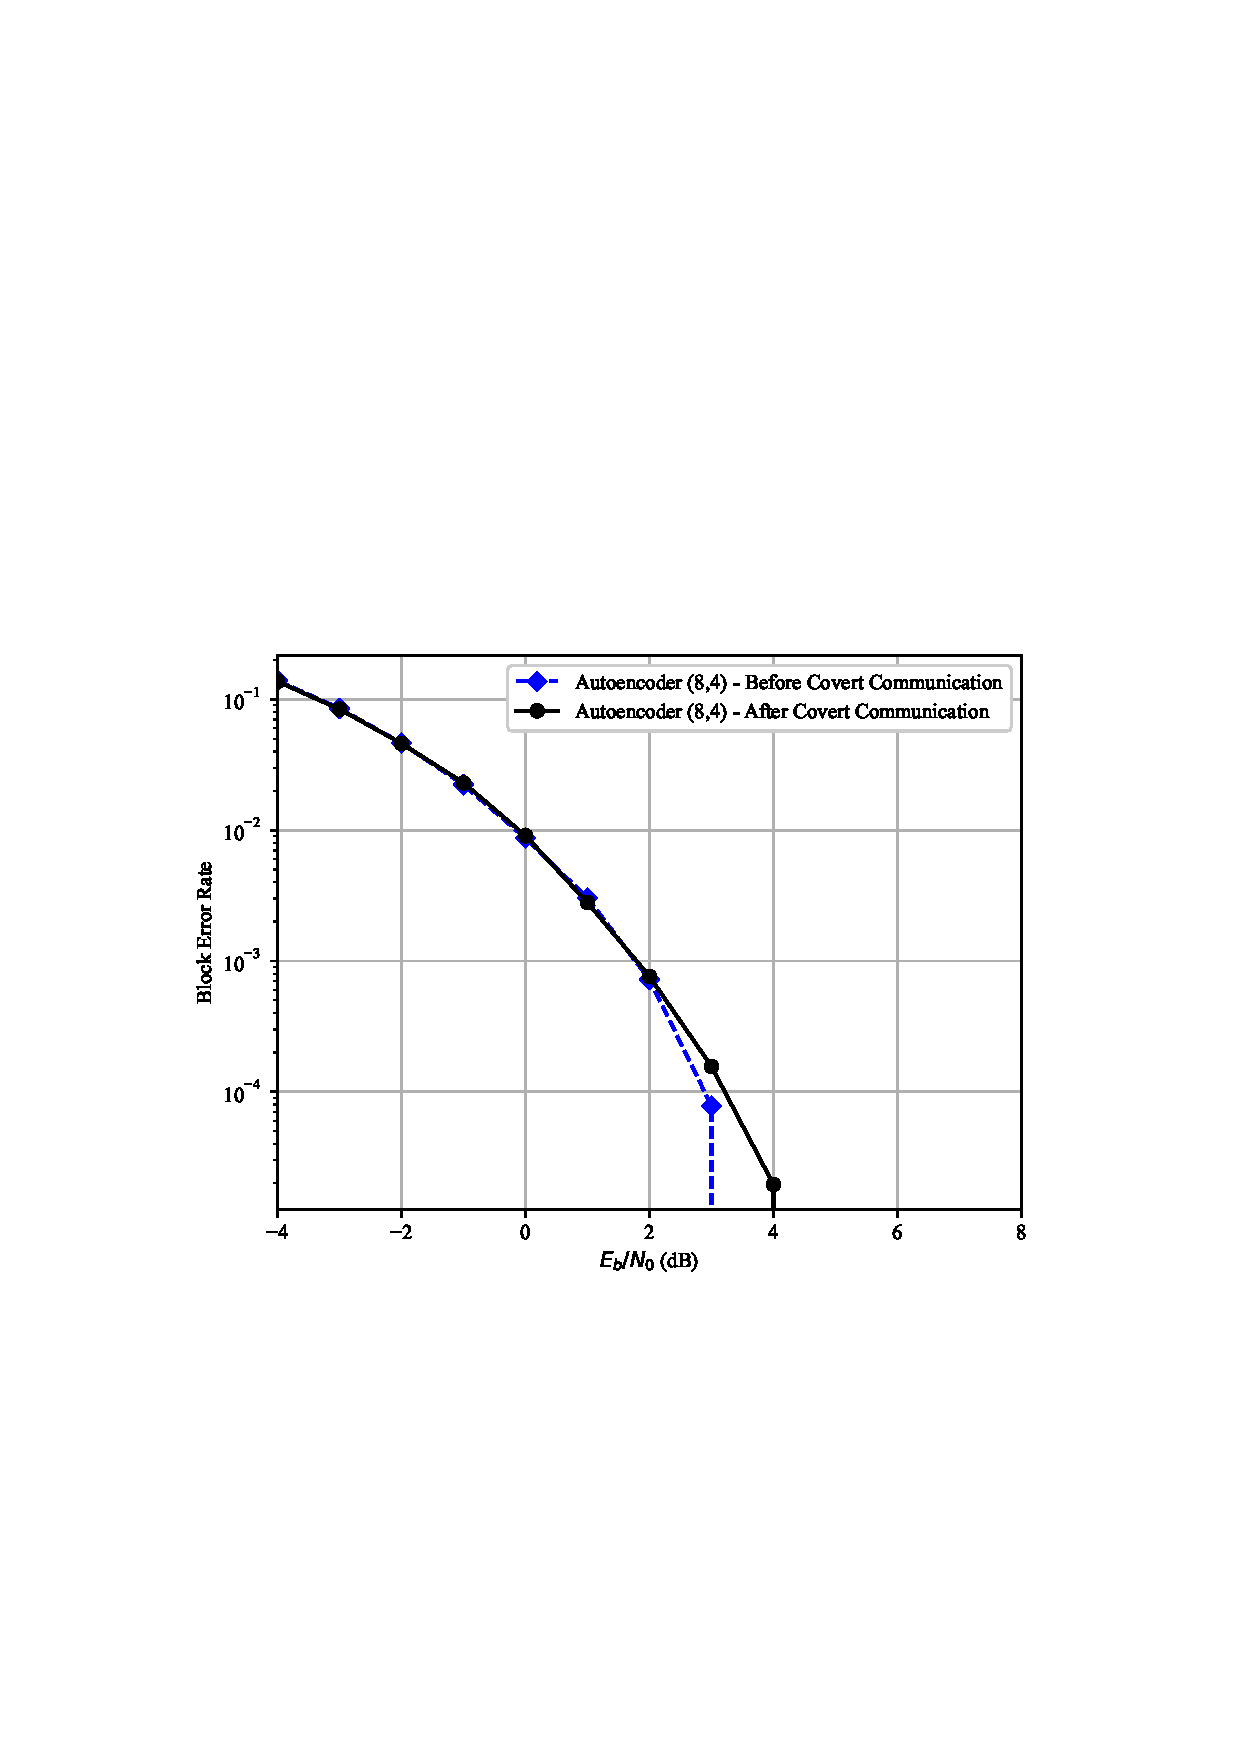
\includegraphics[width=\linewidth]{figs/covert_autoencoder_bler_awgn}
		\caption{Autoencoder's BLER}
		\label{fig:awgn_resutls_ae}
	\end{subfigure}
	\hspace*{\fill}
	\begin{subfigure}{0.28\textwidth}
		\includegraphics[width=\linewidth]{figs/bob_bler_awgn}
		\caption{Bob's BLER}	
		\label{fig:awgn_resutls_bob}
	\end{subfigure}
	\hspace*{\fill}
	\begin{subfigure}{0.28\textwidth}
		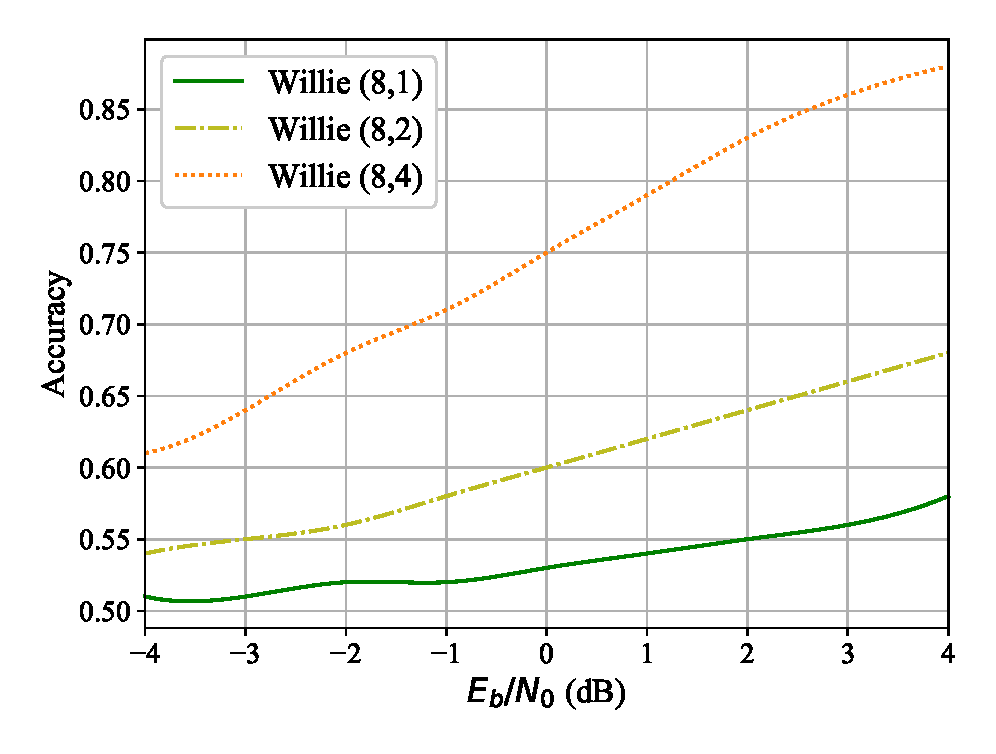
\includegraphics[width=\linewidth]{figs/willie_accuracy_awgn}
		\caption{Willie's accuracy}	
		\label{fig:awgn_resutls_willie}
	\end{subfigure}
	\caption{Trained covert models' performance over AWGN channel for different covert data rates on a range of SNR values.}
	\label{fig:awgn_results}
\end{figure*}
\begin{figure*}[tp!]
	\begin{subfigure}{0.28\textwidth}
		\includegraphics[width=\linewidth]{figs/covert_autoencoder_bler_rayleigh}
		\caption{Autoencoder's BLER}
		\label{fig:rayleigh_resutls_ae}
	\end{subfigure}
	\hspace*{\fill}
	\begin{subfigure}{0.28\textwidth}
		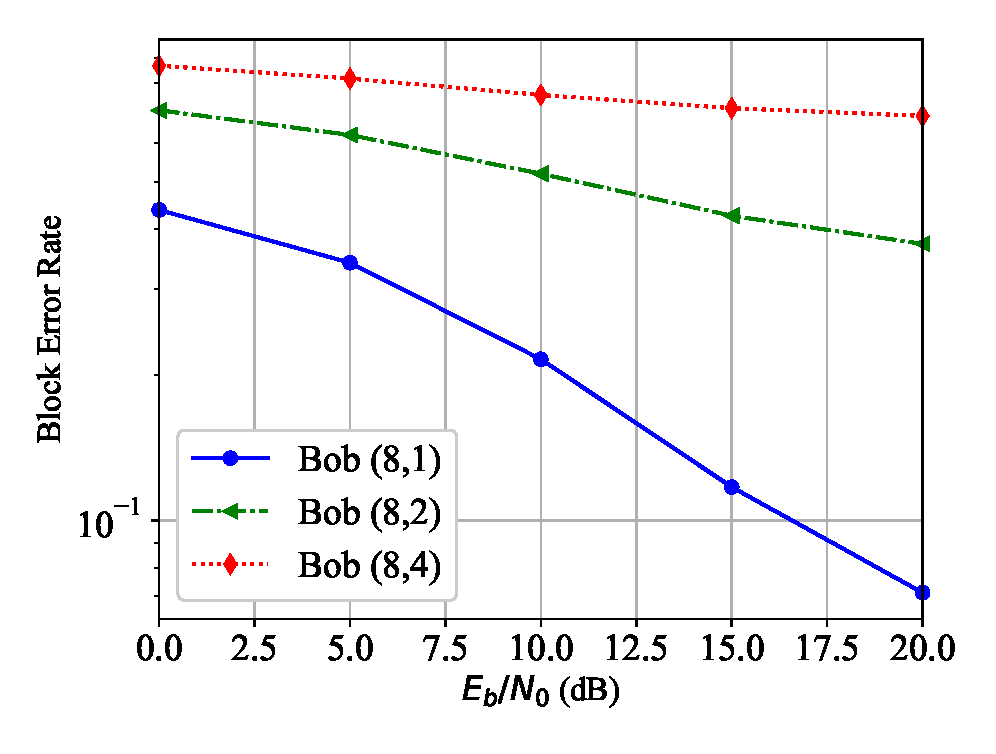
\includegraphics[width=\linewidth]{figs/bob_bler_rayleigh}
		\caption{Bob's BLER}
		\label{fig:rayleigh_resutls_bob}	
	\end{subfigure}
	\hspace*{\fill}
	\begin{subfigure}{0.28\textwidth}
		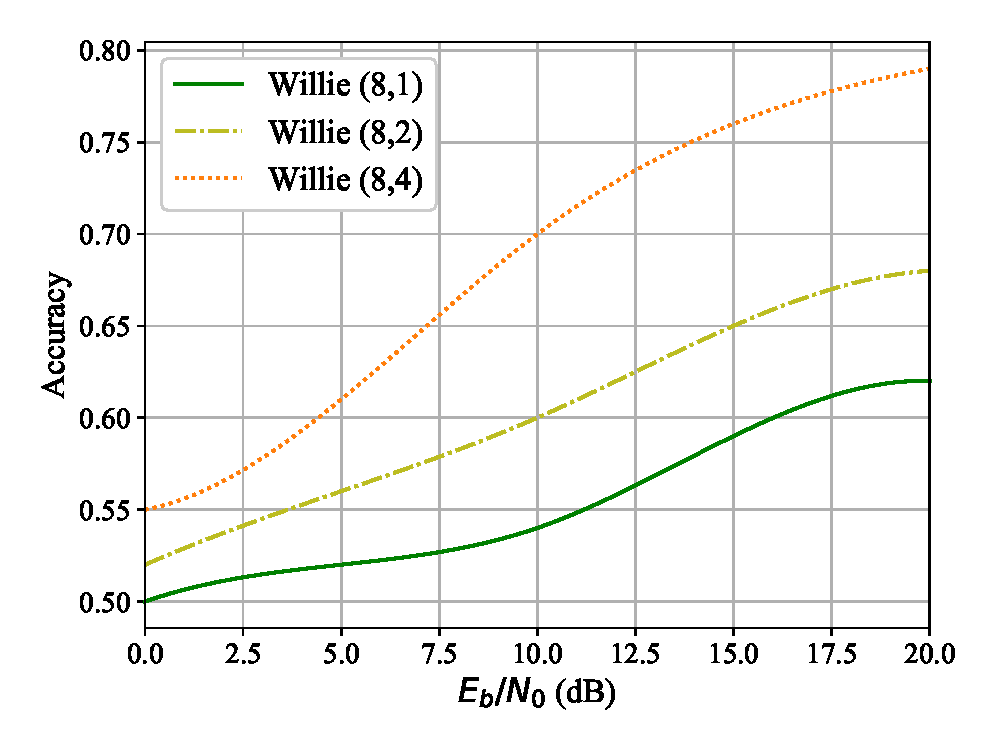
\includegraphics[width=\linewidth]{figs/willie_accuracy_rayleigh}
		\caption{Willie's accuracy}
		\label{fig:rayleigh_resutls_willie}
	\end{subfigure}
	\caption{Trained covert models' performance over Rayleigh fading channel for different covert data rates on a range of SNR values.}
	\label{fig:rayleigh_resutls}
\end{figure*}
\begin{figure*}[tp!]
	\begin{subfigure}{0.28\textwidth}
		\includegraphics[width=\linewidth]{figs/covert_autoencoder_bler_rician}
		\caption{Autoencoder's BLER}
		\label{fig:rician_resutls_ae}
	\end{subfigure}
	\hspace*{\fill}
	\begin{subfigure}{0.28\textwidth}
		\includegraphics[width=\linewidth]{figs/bob_bler_rician}
		\caption{Bob's BLER}
		\label{fig:rician_resutls_bob}	
	\end{subfigure}
	\hspace*{\fill}
	\begin{subfigure}{0.28\textwidth}
		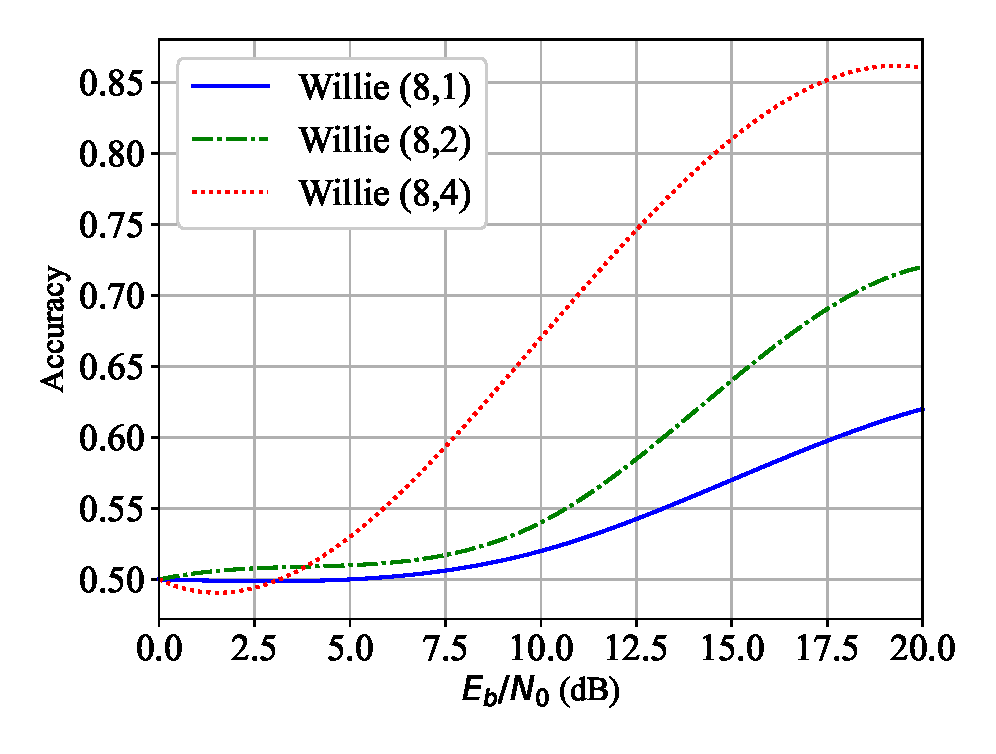
\includegraphics[width=\linewidth]{figs/willie_accuracy_rician}
		\caption{Willie's accuracy}
		\label{fig:rician_resutls_willie}
	\end{subfigure}
	\caption{Trained covert models' performance over Rician fading channel for different covert data rates on a range of SNR values.}
	\label{fig:rician_resutls}
\end{figure*}


\subsection{Covert Model Evaluation Results}
As for the covert models, we evaluate our system's performance on three different channel models of AWGN, Rayleigh fading, and Rician fading for the single-user system, and on two channels of AWGN and Rayeleigh fading for the multi-user one. In all settings, we use the same training procedure, but the network architecture of our covert and autoencoder models in the multi-user system slightly differs from the single-user setting. These differences can be seen in Table \ref{table:multi_models_structure}.

Since each covert message \(m\) has to be paired with a normal message \(s\), we create the covert model's training and testing sets to have the same number of samples as are in the autoencoder's. All models are trained for 5000 epochs using the Adam optimizer in an adversarial training setting. We adjust the importance of each of Alice's objectives by setting \(\lambda_{\mathcal{W}} = 2 \lambda_{\mathcal{B}} = 4 \lambda_{\mathcal{U}}\) for single-user system, and \(\lambda_{\mathcal{W}} = 3 \lambda_{\mathcal{B}} = 6 \lambda_{\mathcal{U}}\) for multi-user system in (\ref{alice_loss}). We have come down to these numbers by running a grid search on these parameters. However, our solution is not limited to these parameters, and in fact, one can use a different set of parameters to emphasize on one specific objective more than the others. In both single-user and multi-user systems, we start the training with a learning rate of 0.001 and gradually halve the learning rate after every 500 epochs. In each epoch, we first update the parameters of Willie's network using (\ref{willie_loss}), then train Alice's network for one step using (\ref{alice_loss}), and eventually optimize Bob's network based on (\ref{bob_loss}). Although we train our autoencoder network on a fixed SNR value, we find our covert scheme performing better when trained on a range of SNR values. We do this by randomly switching the SNR value within a predetermined range after each epoch of training. Training our models this way, not only helps Alice to better preserve the normal communication's accuracy but also makes Bob be able to decode covert messages more accurately on lower SNR values. Accordingly, we start by setting the training SNR to the value that the autoencoder was trained on and incrementally expand the SNR range from both ends until no further improvement is observed. As a result, in the single-user system, we come down to the range of -2dB to 8dB for the AWGN channel and 10dB to 20dB for both the Rayleigh and the Rician fading channels. In multi-user system, the optimal range can be found within 0db to 12db range for AWGN channel, and within 10 to 25db for Rayleigh channel.

\begin{figure*}[tp!]
	\begin{subfigure}{0.28\textwidth}
		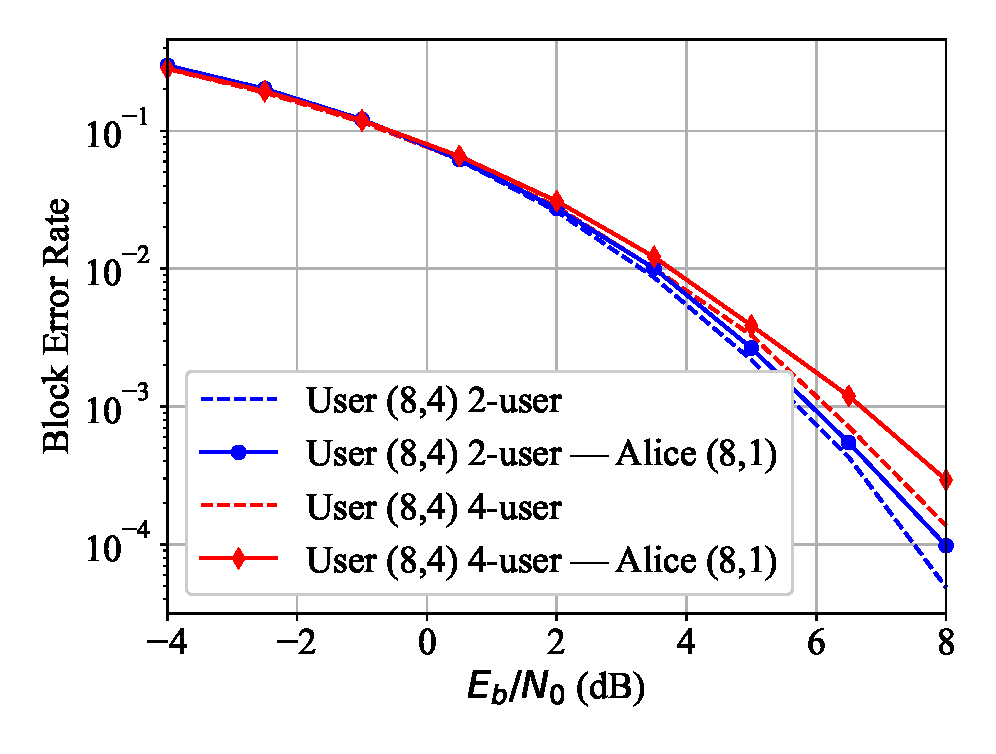
\includegraphics[width=\linewidth]{figs/multi_covert_autoencoder_bler_awgn}
		\caption{Autoencoder's BLER}
		\label{fig:multi_awgn_results_ae}
	\end{subfigure}
	\hspace*{\fill}
	\begin{subfigure}{0.28\textwidth}
		\includegraphics[width=\linewidth]{figs/multi_bob_bler_awgn}
		\caption{Bob's BLER}	
		\label{fig:multi_awgn_results_bob}
	\end{subfigure}
	\hspace*{\fill}
	\begin{subfigure}{0.28\textwidth}
		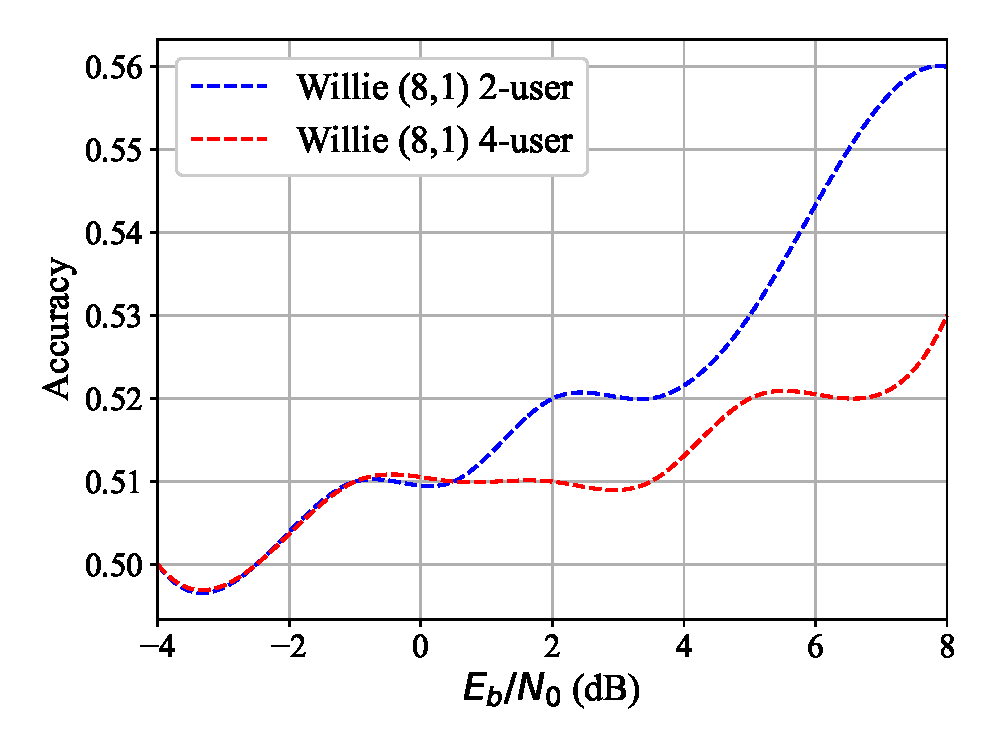
\includegraphics[width=\linewidth]{figs/multi_willie_accuracy_awgn}
		\caption{Willie's accuracy}	
		\label{fig:multi_awgn_results_willie}
	\end{subfigure}
	\caption{Trained covert models' performances over AWGN channel for systems with different numbers of users on a range of SNR values.}
	\label{fig:multi_awgn_results}
\end{figure*}
\begin{figure*}[tp!]
	\begin{subfigure}{0.28\textwidth}
		\includegraphics[width=\linewidth]{figs/multi_covert_autoencoder_bler_rayleigh}
		\caption{Autoencoder's BLER}
		\label{fig:multi_rayleigh_results_ae}
	\end{subfigure}
	\hspace*{\fill}
	\begin{subfigure}{0.28\textwidth}
		\includegraphics[width=\linewidth]{figs/multi_bob_bler_rayleigh}
		\caption{Bob's BLER}
		\label{fig:multi_rayleigh_results_bob}	
	\end{subfigure}
	\hspace*{\fill}
	\begin{subfigure}{0.28\textwidth}
		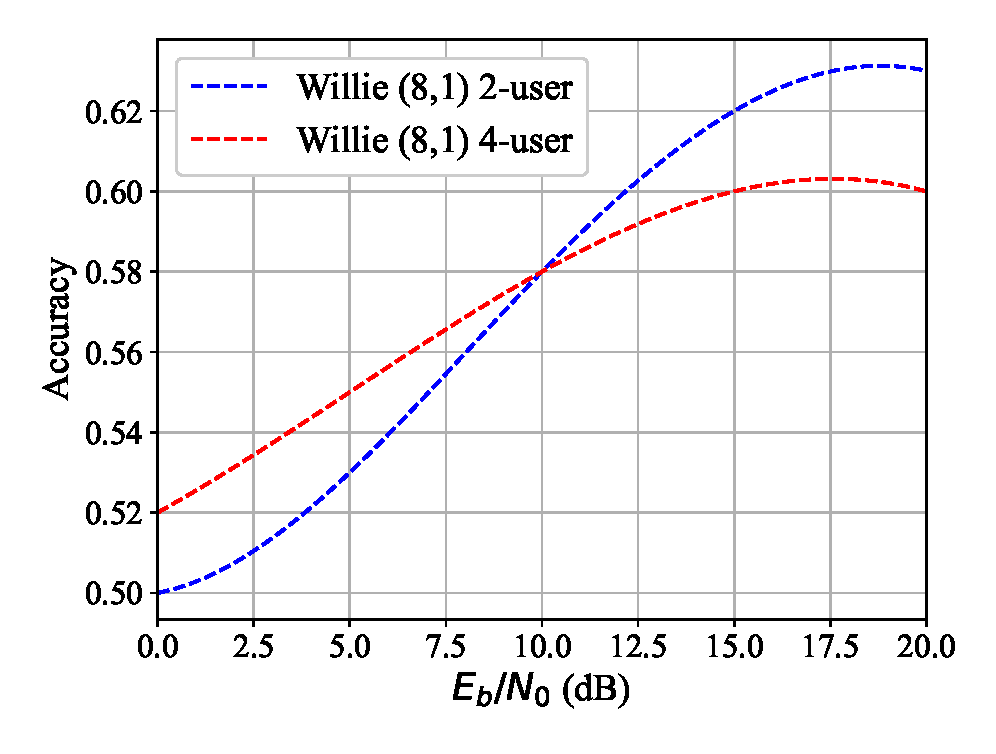
\includegraphics[width=\linewidth]{figs/multi_willie_accuracy_rayleigh}
		\caption{Willie's accuracy}
		\label{fig:multi_rayleigh_results_willie}
	\end{subfigure}
	\caption{Trained covert models' performances over Rayleigh fading channel for systems with different number of users on a range of SNR values.}
	\label{fig:multi_rayleigh_results}
\end{figure*}

Our experiments begin with single-user models. We first evaluate our covert models by sending 1 bit of covert data over 8 channel uses and then gradually increase the number of covert bits to see how increasing the covert data rate affects each component of our covert scheme. We use \(Alice (n,k)\), \(Bob (n,k)\), and \(Willlie (n,k)\) notations to differentiate models operating on different data rates, and the interpretation of them is just the same as autoencoder model's. 

After we evaluated our covert models for covert communication reliability against different covert data rates, in the multi-user system, we now aim to measure the robustness of our covert scheme against number of users. To this end, we evaluate our covert models in multi-user systems comprising of 2 and 4 users. This experiment shows us how adding users to the system affects our covert models performance and whether this has a greater impact on the communication than increasing the covert data rate.

\textbf{Training Procedure}: Figure \ref{fig:traning_progress} shows the progress of each covert actor's accuracy on the test set during the training process for both single-user and multi-user systems. As the training goes on, Bob gradually learns to decode covert messages \(m\) and establishes a reliable communication with Alice. After a few epochs, when the covert communication starts to take form and stabilizes, signals start to deviate from the distribution they had, causing Willie to better detect covert signals. When Willie's accuracy increases, the term \(\mathcal{L}_{\mathcal{W}}\) dominates the other two objectives of Alice's loss function in (\ref{alice_loss}). This causes Alice to gradually sacrifice its accuracy for the sake of undetectability. Soon afterwards, the training process reaches a stable point where neither of the covert models sees any noticeable improvement in their accuracy as the training continues. At the end of the training, \textbf{User's accuracy remains intact, Bob achieves a reliable covert communication accuracy, and Willie stabilizes at around 50$\sim$60\% accuracy which for a binary classifier is almost a random guessing accuracy.}

\textbf{Covert Rate}: Figures \ref{fig:awgn_results}, \ref{fig:rayleigh_resutls}, and \ref{fig:rician_resutls} show our scheme performance for different covert data rates. It also demonstrates how reliable our covert models are against different covert rates. As we expected, covert communication becomes more unreliable, impact on normal communication increases, and detection becomes easier when covert users are sending data at a higher covert rate. From the plots, we can see that sending cover data at higher rates makes the covert communication unreliable. Hence, we proceed with the lowest covert data rate, which is sending 1 bit of data over 8 channel uses, when evaluating our multi-user system.

\textbf{Number of Users}: Figures \ref{fig:multi_awgn_results}, \ref{fig:multi_rayleigh_results} show our final results for two systems of 2-user and 4-user. It demonstrates how numbers of users in the system affects our model's performance. Looking at the multi-user system results and considering the single-user as a 1-user system, it is evident that having more users in the system increases the overall covertness. However, having more users results in less degree of freedom for Alice and Bob to establish their communicate reliably. Thus, their overall covert communication accuracy drops when number of users increases. More users also causes heavier channel interference and consequently, it becomes harder for covert models to establish their covert communication without impacting other normal users.


\textbf{Undetectibility}: Willie's accuracy of detection in percentage can be found in Figures \ref{fig:awgn_resutls_willie}, \ref{fig:rayleigh_resutls_willie}, and \ref{fig:rician_resutls_willie} for single-user, and in Figures \ref{fig:multi_awgn_results_willie}, and \ref{fig:multi_rayleigh_results_willie} for multi-user systems. His detection's performance is evaluated over a range of SNR values for detecting signals as covert and normal. These plots give us some intuition on how probable it will be for our covert signals to be detected by a target detector at each SNR value for different covert rates. In overall, we observe that Willie's detection accuracy in the multi-user system is relatively lower than the single-user system. Comparatively, looking at Willie's performance in the multi-user system, we can see that his accuracy becomes even worse when there are more users in the system.  

Figures \ref{fig:awgn_constellation},\ref{fig:rayleigh_constellation}), and \ref{fig:rician_constellation} compare the constellation cloud of a covert and a normal signal for AWGN, Rayleigh and Rician fading channels in the single-user system. We have marked each symbol of the encoder's output signal \(x\) as black circle points on the constellation diagrams. The red constellation cloud shows how covert signals scatter after going through the channel and the green cloud shows this for normal signals. Since data is sent over 8 channel uses, there are 8 black points on the chart. To be consistent with Willie's accuracy and Bob's error rate for our both channel models, we have set the SNR value to 4dB for the AWGN and 15dB for the Rayleigh fading channel and 8db for the Rician fading channel so that in all channel models, the probability of detection remains relatively the same and the covert communication BLER stays below \(10^{-1}\). This area of operation gives Alice and Bob a relative reliability in their covert communication whilst maintaining their covertness. Looking at these figures, the signal constellation diagrams before and after our covert model being applied shows that Alice has perfectly learned to cloak the covert signals into the distribution of the channel's noise after a successful training procedure.


\begin{figure}[tp!]
	\begin{subfigure}{0.24\textwidth}
		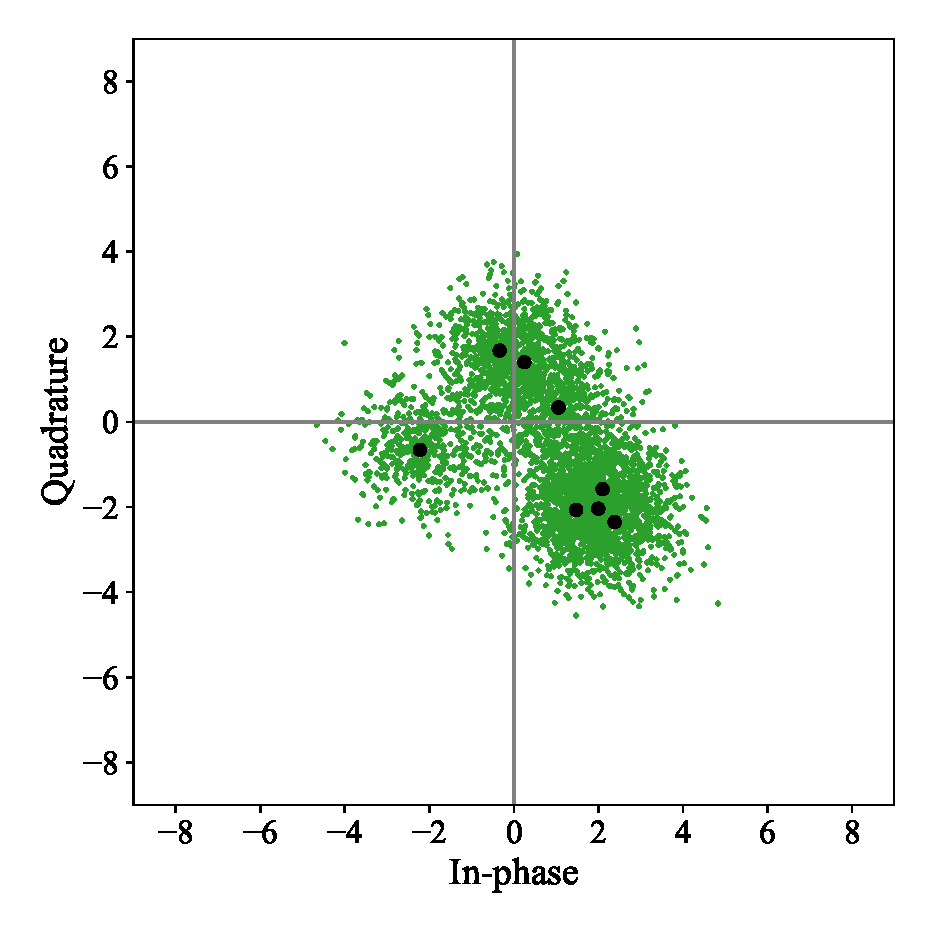
\includegraphics[width=\linewidth]{figs/awgn_normal_constellation}
		\caption{Without covert transmission}
	\end{subfigure}
	\hfill
	\begin{subfigure}{0.24\textwidth}
		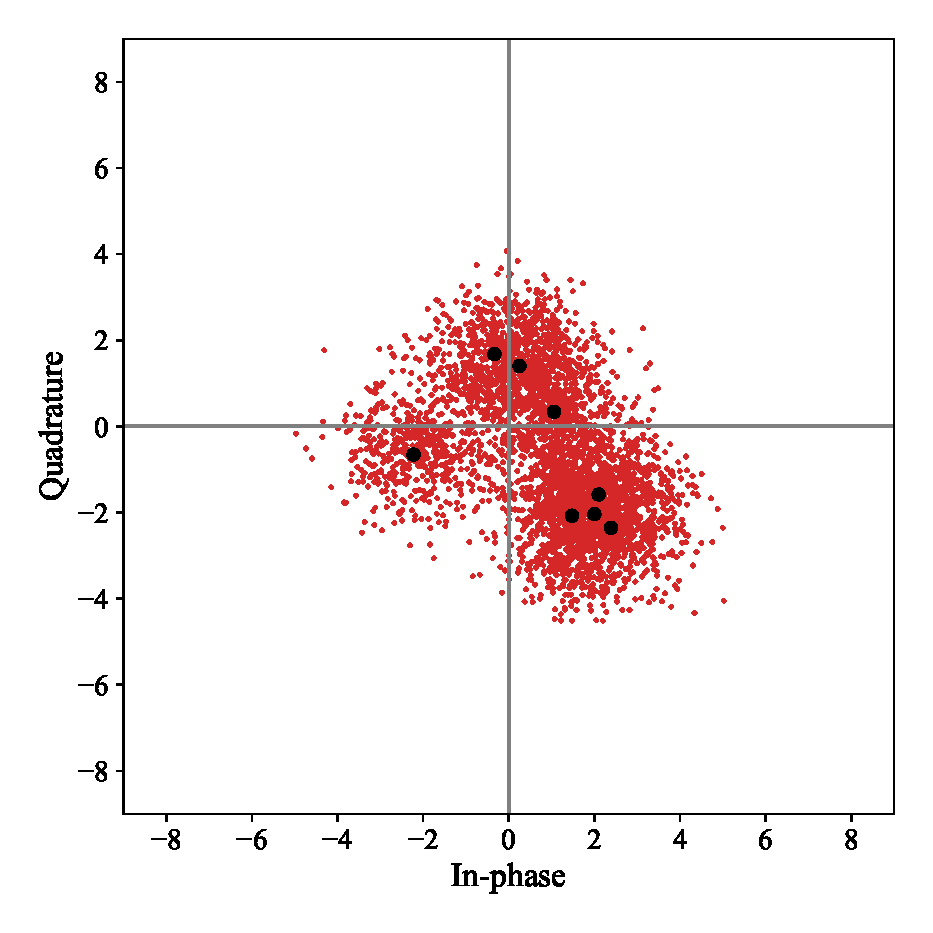
\includegraphics[width=\linewidth]{figs/awgn_covert_constellation}
		\caption{With covert transmission}	
	\end{subfigure}
	\caption{Comparing AWGN channel constellation clouds of a signal before and after our covert scheme being applied.}
	\label{fig:awgn_constellation}
\end{figure}
\begin{figure}[tp!]
	\begin{subfigure}{0.24\textwidth}
		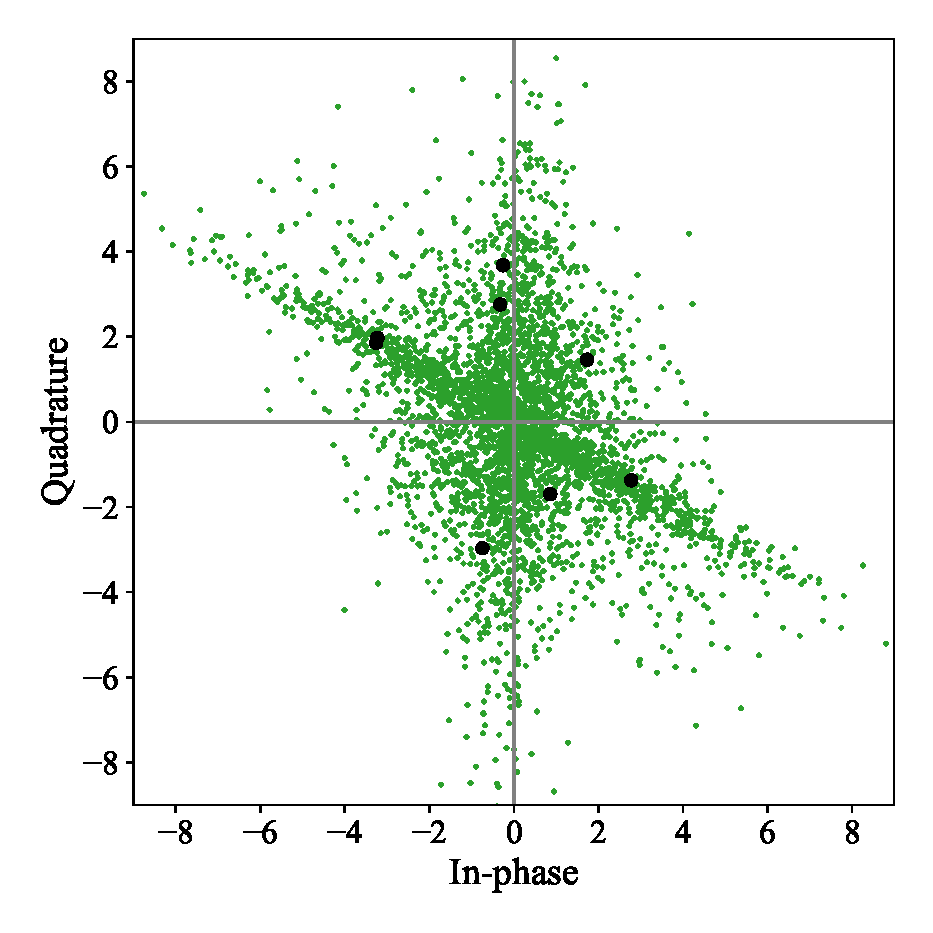
\includegraphics[width=\linewidth]{figs/rayleigh_normal_constellation}
		\caption{Without covert transmission}
	\end{subfigure}
	\hfill
	\begin{subfigure}{0.24\textwidth}
		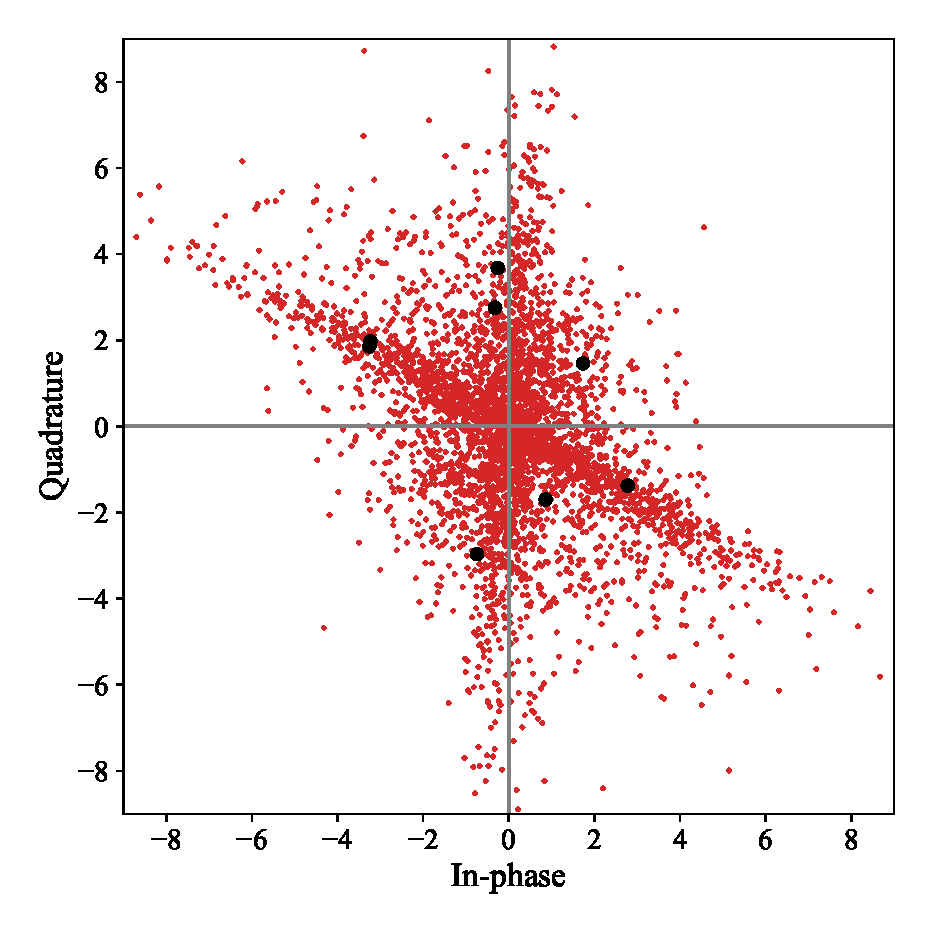
\includegraphics[width=\linewidth]{figs/rayleigh_covert_constellation}
		\caption{With covert transmission}	
	\end{subfigure}
	\caption{Comparing Rayleigh fading channel constellation clouds of a signal before and after our covert scheme being applied.}
	\label{fig:rayleigh_constellation}
\end{figure}
\begin{figure}[tp!]
	\begin{subfigure}{0.24\textwidth}
		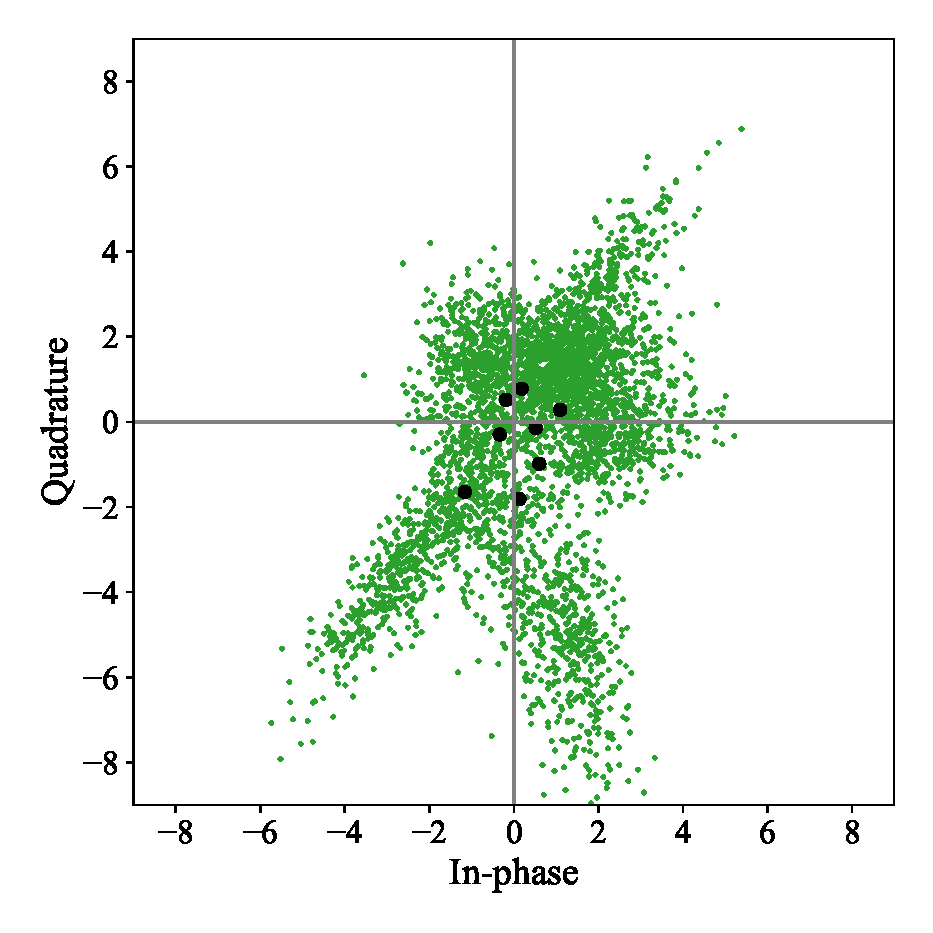
\includegraphics[width=\linewidth]{figs/rician_normal_constellation}
		\caption{Without covert transmission}
	\end{subfigure}
	\hfill
	\begin{subfigure}{0.24\textwidth}
		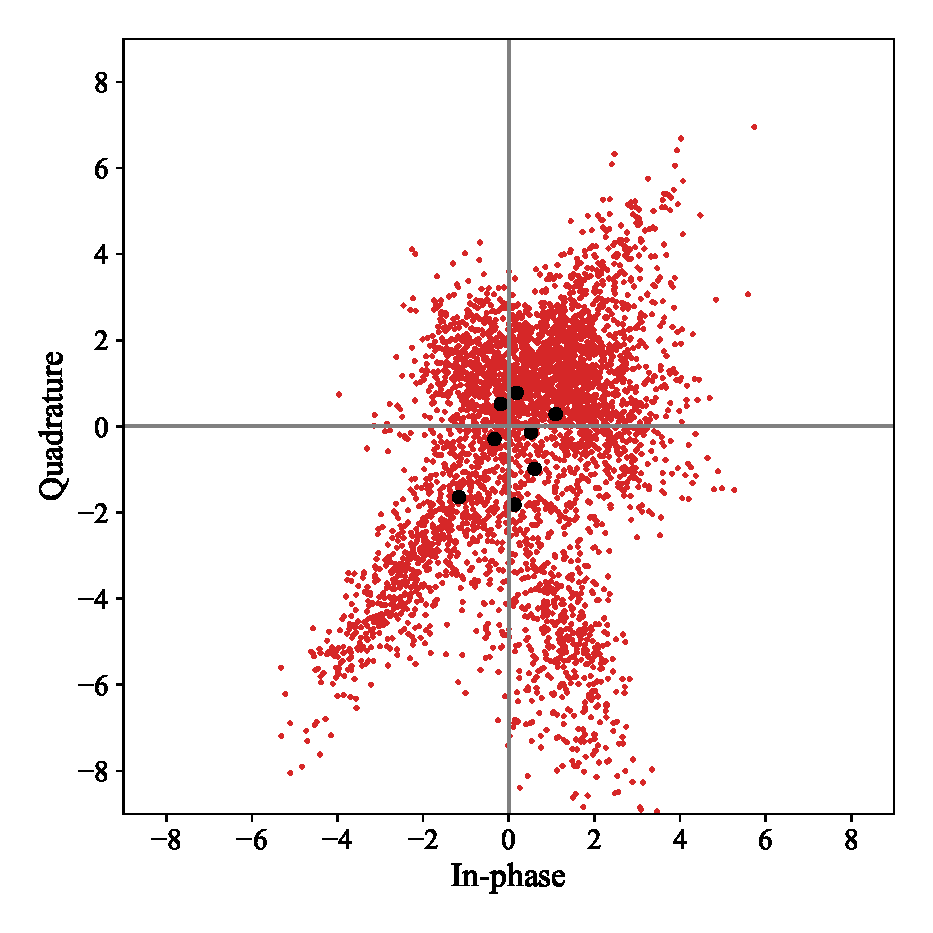
\includegraphics[width=\linewidth]{figs/rician_covert_constellation}
		\caption{With covert transmission}	
	\end{subfigure}
	\caption{Comparing Rician fading channel constellation clouds of a signal before and after our covert scheme being applied.}
	\label{fig:rician_constellation}
\end{figure}
